\chapter{Background}
\label{chapter:background}
\thispagestyle{myheadings}

\graphicspath{{1a_background/Figures/}}

This work was motivated by the desire to scale microfluidic devices using automation techniques derived from the evolution of microelectronics. The emergence of microfluidic large scale integration (mLSI) resulted in the formulation of methods to manage complexity in design and fabrication. These methods often draw analogies with design and computation using microelectronics \cite{minhass2013}. Unfortunately, these efforts can often be disjointed --- automated design methods rely on manually-intensive fabrication efforts, or vice versa. What results from a unification of these efforts is a design-to-device workflow made possible by a new microfluidic fabrication framework, MakerFluidics, presented in Chapter \ref{chapter:mf}. This framework better utilizes automation via computer-aided manufacturing (CAM) at a lower cost in both time and money when compared to the traditional fabrication framework, namely soft lithography, the background for which is provided in Section \ref{ssec:backgroundSL}.

MakerFluidics was proven viable by designing, fabricating, and controlling a system of novel microfluidic primitive aimed at providing an element of programmability in continuous-flow microfluidic devices, a problem better motivated in Section \ref{sec:backgroundCFRouting}. 

Finally, the MakerFluidics framework sought immediate experimental relevance by partnering with industry to push the state of the art in bacterial identification and antimicrobial susceptibility testing (IDAST). A solution to this problem would delay the post-antibiotic era \cite{alanis2005resistance} and save tens of thousands of lives per year \cite{world2004world}. MakerFluidics was responsible for optimizing the sample purification process, which involves separating bacteria from blood in a microfluidic chip using acoustic manipulation. The purified bacterial sample could then be used in a downstream assay where pathogen IDAST is performed. Background information for IDAST and acoustic manipulation is provided in Section \ref{sec:cellSep}.

\section{Microfluidic Fabrication Using Multi-Layer Soft Lithography}
\label{ssec:backgroundSL}
Soft lithography was adopted as the traditional method of fabricating large-scale microfluidics based on the demonstrated success of photolithography in fabricating microelectronics \cite{whitesides2006}. A typical device design utilizes two layers: flow and control. The flow layer is the layer through which your fluids (i.e., samples of interest) flow. The control layer is responsible for controlling fluids on the flow layer via pneumatic valving \cite{unger2000}. Each layer requires its own replica mold. A detailed description of microfluidic fabrication using multi-layer soft lithography is provided in a number of reviews \cite{duffy1998}\cite{sia2003}\cite{weibel2007}. A brief overview of the three main steps to this process are outlined below.

\subsection{Replica Mold Fabrication}
A light-sensitive material called a photoresist is applied to the surface of a silicon wafer using a spin coater. The wafer is then baked in an oven to remove solvents and bubbles from the photoresist that may have been introduced during application. The device design is printed onto an overhead transparency, which is then laid upon the coated silicon wafer. The stack containing the silicon wafer, photoresist, and transparency are exposed to UV light using a piece of equipment called a mask aligner. This process must take place within the confines of a cleanroom as stray UV light or physical particles (e.g., lint, dust, etc.) can introduce erroneous features into the design. Upon completion of UV exposure the mask is placed in a developing agent, after which the silicon is washed to produce the replica mold.

\begin{figure}[h]
  \begin{minipage}[t]{0.99\linewidth}\centering
    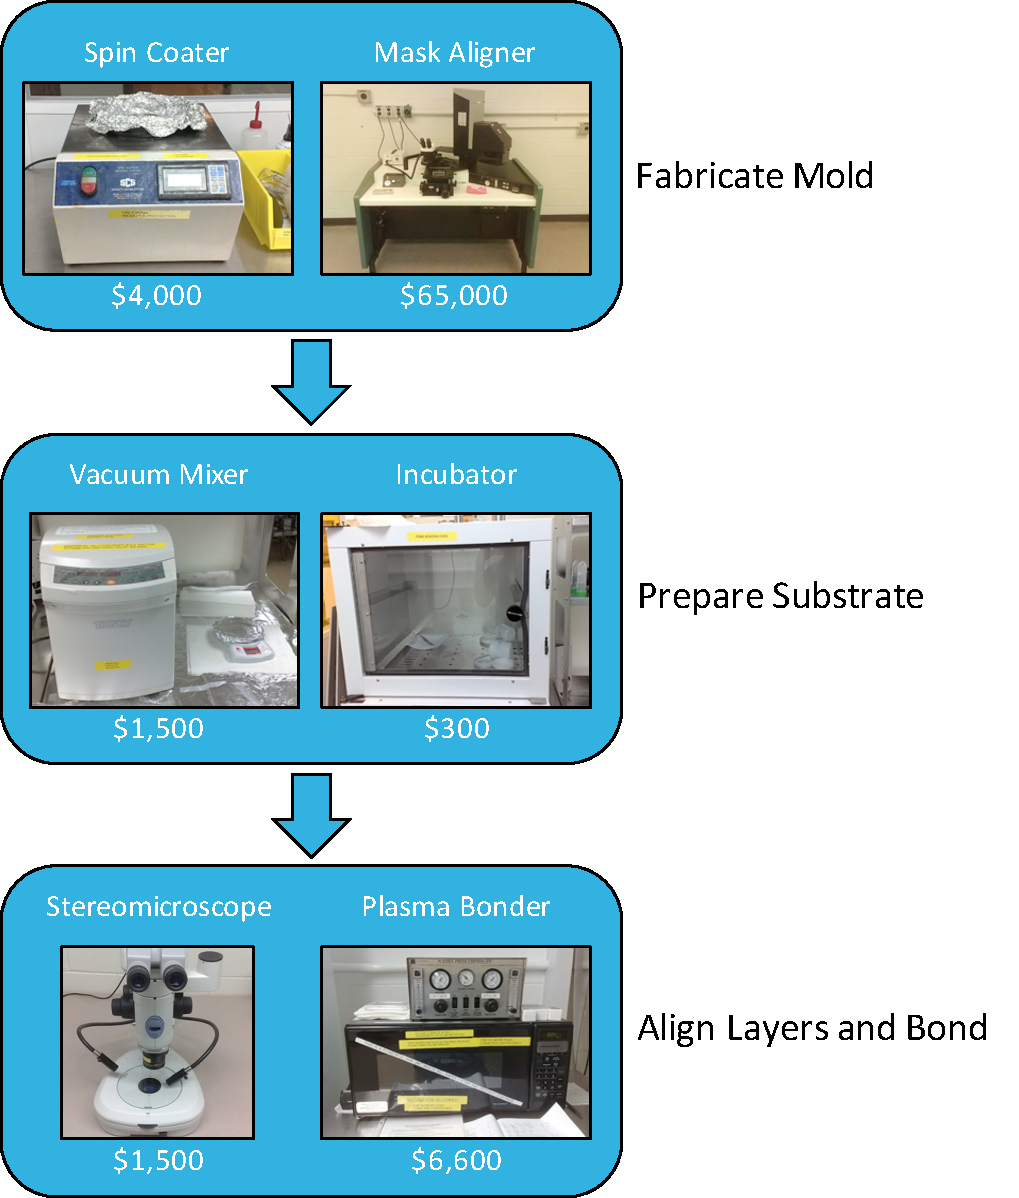
\includegraphics[width=6cm]{equipSoftLith.pdf}
    \medskip
  \end{minipage}\hfill
  \caption[Specialized equipment required to performform soft lithography]{Microfluidic fabrication via multi-layer soft lithography requires about \$80,000 in specialized equipment, not accounting for infrastructure, personnel, maintenance, or training. Cost estimates based on company quotes.}
    \label{fig:equipSoftLith}
\end{figure}


\subsection{Preparation of Substrate}
The substrate of choice for multi-layer soft lithography is a silicon elastomer known as polydimethylsiloxane (PDMS). This material is the result of combining a cross-linker and gel in a vacuum mixer, ensuring that no bubbles are present in the mixture. The flow layer is produced by carefully spin coating PDMS upon the silicon wafer ensuring that the features are fully immersed by the uncured elastomer. Excess elastomer is spun on top of the immersed features, which will result in the formation of a membrane used by the control layer to valve the flow of fluids. Unlike the flow layer, the control layer does not require the formation of a membrane of specified thickness, thus less precision is required for PDMS-coating the control layer's silicon mold. After coating, the PDMS for each layer is cured in an incubator.

\subsection{Alignment of Layers and Bonding}
After removing the PDMS from the silicon mold, the flow and control layers must be bonded together. This is often accomplished by modifying the surface chemistry of the PDMS using a plasma treatment. Each layer is placed, bonding-side-up in a plasma bonder. After removing the PDMS layers from the plasma bonder, the flow layer must be perfectly aligned with the control layer as the pneumatic valves must overlay their corresponding fluidic channels. This is accomplished by hand under a microscope and must be completed within a finite amount of time (often minutes) before the plasma treatment wears off. This process is then repeated to seal the fluidic layer to a piece of glass. 

\section{The Microfluidic--Microelectronic Analogy}
\label{sec:backgroundCFRouting}

It is difficult to imagine a computer engineer having to create a VLSI layout and fabricate an ASIC every time they wanted to run a C program. While there will always be a place for custom circuit design in the world of digital electronics one basic tenant of digital design, namely abstraction, requires that it remain very much the exception rather than the rule. Unfortunately for the experimentalist, this is not the case in the field of microfluidics. The creation of custom, ``one-off'', designs for individual microfluidic experiments, no matter how user-friendly the corresponding CAD software is, could be is what is keeping the productivity of mLSI chips from achieving that of its silicon counterparts. Since Thorsen \emph{et al.} successfully integrated thousands of micromechanical valves in 2002 \cite{thorsen2002}, academic researchers have attempted to manage exponentially greater complexity in microfluidic design via the introduction of new design methodologies that attempt to introduce ``top-down'' specificity and move away from a ``bottom-up'' design philosophy \cite{minhass2013}\cite{melin2007}\cite{minhass2012} yet microfluidic experimentalists still find themselves in front of an oven baking a photoresist until it ceases to be sticky. 

Managing complexity is a necessary craft in that it allows the engineer to design complicated systems without becoming overwhelmed by details. The art of managing complexity in digital electronics design is  a mature process relative to that found in microfluidics. This is evident by the existence of larger scales of integration \emph{in silico}, such as VLSI, and by microfluidic efforts to create tools that mirror the design-to-execution workflow found in electronic computing. Examples of such tools are Micado, for automation of control layer routing \cite{amin2009}, and BioStream \cite{thies2008}, which could serve as the cornerstone of true experimental automation and will be described in the subsequent section. It could serve as a useful exercise to emphasize one methodology used to design and fabricate microelectronics while managing complexity and then contrast this principle with the current state of microfluidic design. There are few better places to find fundamental digital design practices than in introductory textbooks, one of which lists abstraction as the most important element of managing complexity \cite{Harris+Harris}.

If the goal is true experimental automation, then the expensive and time-consuming fabrication step should be removed from the work flow for the majority case as it is for electronic computation. Often, academic papers delving into the relm of mLSI begin by presenting an analogy between microfluidic LSI and LSI found in digital electronics. This research analogy seems strange as computer engineers can be productive using programmable tools (e.g., personal computers, Field Programmable Gate Arrays (FPGA), etc.) without having to know how to wash chemical from printed circuit boards (PCBs), use CAD tools to layout application specific integrated circuits (ASICs), or enlist the aid of experts in fabrication who can. Thus, the \emph{in silico} analogy does not hold when applied to the common-use case: that of the individual scientist or engineer.

Chapter \ref{chapter:xposer} outlines a novel primitive for continuous-flow microfluidics aimed at unlocking elements of programmability in continuous-flow devices. It analyzes and solves microfluidic design challenges using tools for automated design and control, ultimately providing a solution that would allow the microfluidic experimentalist to be one step closer to realizing the productivity potential of true large-scale integration. 

\subsection{Microfluidic Design Tools}
\label{ssec:DesignTools}

Abstraction works by placing the user at only the highest level relevant to the computation being performed and masking all underlying details. It can, therefore, be contended that functionally complete automation of microfluidic experiments implies placing the scientist at only the highest levels of abstraction and masking all underlying details. Currently, even the best efforts in microfluidic tools only remove intermediate levels of abstraction, while exposing the scientist to the highest \textbf{and lowest} levels. Imagine if the only output of a C program were a circuit schematic that must first be built in order to obtain the result of the program. The use of the term ``working levels'' of complexity implies that the person operating within that layer need not concern themselves with the details of a lower layer, as such requirements would ultimately defeat the purpose of abstraction. Lower levels of detail are said to be ``abstracted'' away when their use is considered automatic. However, designers of systems residing in one particular abstraction layer should have an understanding of how their design decisions affect the layers immediately above and below the working layer, such as a C programmer understanding the nature of an address space \cite{Harris+Harris}. Theis \emph{et al} advocate for the creation of abstraction layers in microfluidics similar to that found in electronic computing \cite{thies2008}. These layers achieve success by focusing on three basic fluidic operations: mixing, transport and storage. Their BioStream protocol is a good first step in decoupling microfluidic architecture from biological computation by providing a common language for describing an experimental protocol. BioStream served initially as a standard language for reporting biological protocols but expanded to an end-to-end system that effectively describes biological protocols within the BioStream Fluidic ISA and executes them at the hardware level independent of microfluidic chip microarchitecture \cite{thies2008}. BioStream, however, does not fully address a functional purpose of abstraction, which is to provide automation, but it does accomplish a very important step the authors describe as a ``division of labor'' between the biology and microfluidic experts. 
There is, and probably always will be, a place in digital electronics for PCB design and ASIC fabrication. However, before an engineer decides to begin the process of building a custom PCB or layout a new ASIC they should first consider how their deisgn decision addresses the productivity gap. In order to proceed, a working definition of the term ``productivity'' must be presented. Process and requirements engineers \cite{Review_ProcessEngr} have defined productivity strictly in terms of hours saved \cite{CostBenefit_hours}, as a function of on-time delivery \cite{OnTimeDelivery} or as some measure of quality \cite{Quality}. This paper will define the productivity of a particular method as the number of hours saved through the implementation of a particular process.

Device fabrication is not a task oft performed by a computer scientist. Rather, a computer scientist spends many hours debugging a program such that it runs reliably and correctly within the confines of a particular ISA. This exemplifies the nature of design discipline. It is well-within the realm of possibility for a computer engineer to give up debugging a program and reach for a CAD tool, with which to build a custom chip designed for their particular purposes. That scenario would only make sense if the final custom-fabricated solution could overcome the extremely large gap in productivity inherent to designing and fabricating it. The amount of lead-time required to design and build an ASIC or PCB could significantly outweigh the benefits of having a single custom-chip to use only in very specific circumstances and only within that one engineer's lab. Why then is this practice deemed acceptable in microfluidics?

Even attempts to create some framework for flow-based microfluidic design, such as a common microfluidic ISA\cite{amin2009} or predefined software modules \cite{soe2013} are still, fundamentally, design methods for chip fabrication. Microfluidic chip fabrication is a highly unproductive in that it requires many hours to design and build a device incapable of performing diverse and repeatable experiments. Fortunately for the computer engineer there exists other prototyping options besides PCBs and ASICs, such as the use of a field programmable gate array (FPGA) or microcontroller. The microfluidic experimentalist is left with only one prototyping option that almost always requires some level of device
fabrication.


It is difficult to imagine a computer engineer having to create a VLSI layout and fabricate an ASIC every time they wanted to run a C program. While there will always be a place for custom circuit design in the world of digital electronics, the basic tenants of digital design require that it remain very much the exception rather than the rule. Unfortunately for the experimentalist, this is not the case in the field of continuous-flow microfluidics. The creation of custom, ``one-off'', designs for individual microfluidic experiments, no matter how user-friendly the corresponding CAD software is, could be is what is keeping the productivity of mLSI chips from achieving that of its silicon counterparts. Since Thorsen \emph{et al.} successfully integrated thousands of micromechanical valves in 2002 \cite{thorsen2002}, academic researchers have attempted to manage exponentially greater complexity in microfluidic design via the introduction of new design methodologies that attempt to introduce ``top-down'' specificity and move away from a ``bottom-up'' design philosophy \cite{minhass2013}\cite{melin2007}\cite{minhass2012} yet microfluidic experimentalists still find themselves in front of an oven baking a photoresist until it ceases to be sticky. 

If the goal is true experimental automation, then the expensive and time-consuming fabrication step must be removed from the work flow for the majority case as it is for electronic computation. Often, academic papers delving into the relm of mLSI begin by presenting an analogy between microfluidic LSI and LSI found in digital electronics. This analogy seems strange as computer engineers can be productive without having to know how to wash chemical from printed circuit boards (PCBs), use CAD tools to layout application specific integrated circuits (ASICs), or enlist the aid of experts in fabrication who can. Thus, the \emph{in silico} analogy does not hold when applied to the common-use case: that of the individual scientist or engineer. Why is that? This paper will provide a possible answer via a historical analysis of the emergence of digital electronics design and highlight instances where microfluidics deviated, resulting in the current design topology seen today. It will also analyze various attempts to rectify microfluidic design challenges using various computer-aided tools and possibly provide the missing element that would allow the microfluidic experimentalist to be one step closer to realizing the productivity potential of true large-scale integration. 



\section{Pathogen Identification and Antibiotic Susceptibility Testing}
\label{sec:cellSep}

The World Health Organization has listed infectious disease as the second leading cause of death worldwide \cite{world2004world}. Multiple days of lab processing is currently required to determine a particular bacterial identity and its susceptibility to a particular antibiotic. In the interim, infections are often treated using broad-spectrum antibiotics, which has resulted in the rise of antibiotic resistance \cite{laxminarayan2013antibiotic}. The ultimate goal of the IDAST program at the Charles Stark Draper Laboratory is to determine information regarding a pathogens phenotype and antibiotic susceptibility at the point of care within the time-frame of a single visit to the doctor. This is performed using a multi-staged approach shown in Figure \ref{fig:idastFlow}.

\begin{figure}[h]
  \begin{minipage}[t]{0.99\linewidth}\centering
    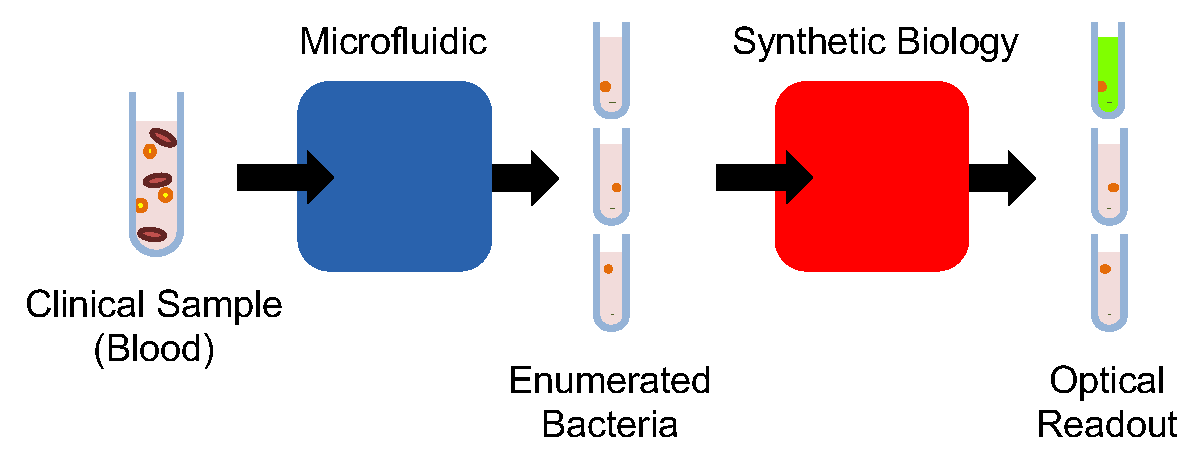
\includegraphics[width=13cm]{idastFlow.pdf}
    \medskip
  \end{minipage}\hfill
  \caption[System-Level View of IDAST]{IDAST is performed using a microfluidic device for sample processing followed by a proprietary synthetic-biological approach resulting in an optical readout.}
    \label{fig:idastFlow}
\end{figure}


